\lcTex{%
  \newlength{\widthExtra}\setlength{\widthExtra}{1.1cm}
  \newlength{\widthLineReal}\setlength{\widthLineReal}{\linewidth}
  \addtolength{\widthLineReal}{-\widthExtra}
  \newlength{\minipageSpace}\setlength{\minipageSpace}{0.2cm}

  \newlength{\widthLeft}
  \newlength{\widthRight}
}

\newcommand{\reals}{{\rm I\!\hspace{-0.025em} R}}
\newcommand{\calC}{{\cal C}}
\newcommand{\calA}{{\cal A}}
\newcommand{\eps}{{\varepsilon}}
\newcommand{\dcel}{{\sc Dcel}}
\newcommand{\naive}{na\"{\i}ve}
\newcommand{\kdtree}{{\sc Kd}-tree}
\newcommand{\Cpp}{{C}{\tt ++}}

% ====================
\section{Introduction}
\label{bobs_sec:intro}
% ====================

\begin{figure}[!htp]
\begin{center}
\begin{ccTexOnly}
  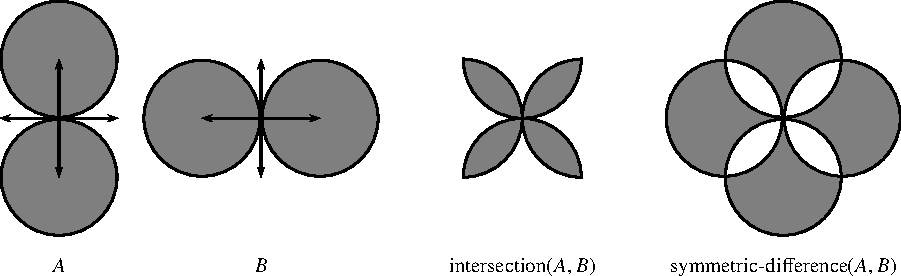
\includegraphics{Boolean_set_operations_2/fig/teaser}
\end{ccTexOnly}
\label{fig:teaser}
\begin{ccHtmlOnly}
  <p><center>
    <img src="./fig/teaser.gif" border=0 alt="Boolean Set-Operations">
  </center>
\end{ccHtmlOnly}
\caption{Examples of Boolean set-operations on general polygons.} 
\end{center}
\end{figure}

This package consists of the implementation of Boolean set-operations
on point sets bounded by $x$-monotone curves\footnote{A continuous
planar curve $C$ is {\em $x$-monotone} if every vertical line intersects it at
most once. We also allow vertical line segments, which are considered
{\em weakly} $x$-monotone.} in 2-dimensional Euclidean space. In particular,
it contains the implementation of {\em regularized} Boolean set-operations,
intersection predicates, and point containment predicates.
Figure~\ref{fig:teaser} shows simple examples of such operations.

A regularized Boolean set-operation $\mbox{op}^*$ can be obtained by
first taking the interior of the resultant point set of an {\em ordinary}
Boolean set-operation $(P\ \mbox{op}\ Q)$ and then by taking the
closure~\cite{cgal:h-sm-04}. That is,
$P\ \mbox{op}^*\ Q = \mbox{closure}(\mbox{interior} (P\ \mbox{op}\ Q))$.
Regularized Boolean set-operations appear in Constructive Solid
Geometry (CSG), because regular sets are closed under regularized
Boolean set-operations, and because regularization eliminates lower
dimensional features, namely isolated vertices and antennas, thus
simplifying and restricting the representation to physically meaningful
solids. Our package provides regularized operations on polygons and
general polygons, where the edges of a general polygon may be
general $x$-monotone curves, rather than being simple line segments.
Ordinary Boolean set-operations, which distinguish between the
interior and the boundary of a polygon, are not implemented within this
package. The \ccc{Nef_2} package supports these operations for (linear)
polygons; see Chapter~\ref{chap:nef_2}.

In the rest of this chapter we use --- unless otherwise stated --- the
traditional notation to designate regularized operations; e.g., $P \cap Q$
means the {\em regularized} intersection of $P$ and $Q$.

A polygon $P$ is said to be {\em simple} (or Jordan) if the only
points of the plane belonging to two polygon edges of $P$ are the
polygon vertices of $P$. Namely, the polygon edges are pairwise
disjoint in their interior. Such a polygon has a well-defined interior
and exterior and is topologically equivalent to a disk. A polygon in our
context must be simple and its vertices must be ordered in a
counterclockwise direction around the interior of the polygon.
 
\lcTex{%
  \setlength{\widthRight}{1.4cm}
  \setlength{\widthLeft}{\widthLineReal}
  \addtolength{\widthLeft}{-\widthRight}
  \begin{minipage}{\widthLeft}
}
\label{fig:non_strictly_simple_polygon}
\begin{ccHtmlOnly}
  <p><center>
    <img src="./fig/non_strictly_simple.gif" border=0 alt="A non strictly simple polygon" align=right>
  </center>
\end{ccHtmlOnly}
The counterclockwise cyclic sequence of alternating polygon edges and
polygon vertices is referred to as the polygon {\em boundary}.
A polygon whose boundary contains the same vertex twice or more is connected
and simple but not necessarily strictly simple, such as the polygon depicted
on the right.  We extend the notion of a polygon to a point set in $\reals^2$
that has  a topology of a polygon and its boundary edges must map to
$x$-monotone curves, and refer to it as a {\em general polygon}. We
sometimes use the term {\em polygon} instead of general polygon for
simplicity hereafter.
\lcTex{%
  \end{minipage}\hspace{\minipageSpace}
  \begin{minipage}{\widthRight}
    \begin{center}
    
\includegraphics{Boolean_set_operations_2/fig/non_strictly_simple}
    \end{center}
%    A non strictly simple polygon.
  \end{minipage}
}

Our package supports the following Boolean set-operations on two point
sets $P$ and $Q$ that are comprized of general polygons:
\begin{description}
\item[Intersection] computes the intersection $R = P \cap Q$.
\item[Join] computes the union $R = P \cup Q$.
\item [Difference] computes the difference $R = P \setminus Q$.
\item [Symmetric Difference] computes the symmetric
  \ccHtmlNoLinksFrom{difference} $P = P \oplus Q = (P \setminus Q) \cup (Q \setminus P)$.
\item[Complement] computes the complement
  \lcTex{$R = \overline{P}$.}
  \lcRawHtml{<i>R = <span style="text-decoration: overline;">P</span>.</i>}
\item [Intersection predicate] tests whether the two sets $P$ and $Q$
  overlap, distinguishing three possible scenarios: (i) the two sets
  intersect on their interior (that is, their regularized intersection
  is not empty $P \cap Q \neq \emptyset$); (ii) the boundaries of two
  sets intersect but their interiors are disjoint; namely they have a
  finite number of common points or even share a boundary curve (still
  in this case $P \cap Q = \emptyset$; and (iii) the two sets are
  disjoint.
\end{description}
In general, the set $R$, resulting from a regularized Boolean
set-operation, is considered as being a closed point-set.

In the rest of this chapter we review the Boolean set-operations package
in more depth. In Section~\ref{bops_sec:bops_lin} we focus on Boolean 
set-operations on linear polygons, introducing the notion of polygons with 
holes and of a general polygon set. Section~\ref{bops_sec:bops_gen}
introduces general polygons.
We first discuss polygons whose edges are either line segements or circular
arcs and then explain how to construct and use general polygons whose edges
can be arbitrary $x$-monotone curves.

% =================================================
\section{Boolean Set-Operations on Linear Polygons}
\label{bops_sec:bops_lin}
% =================================================

The basic library of \cgal\ includes the \ccc{Polygon_2<Kernel,Container>}
class-template that represents a linear polygon in the plane. The
polygon is represented by its vertices stored in a container of
objects of type \ccc{Kernel::Point_2}. The polygon edges are line
segments (\ccc{Kenrel::Segment_2} objects) between adjacent points in
the container. By default, the \ccc{Container} is a vector of
\ccc{Kernel::Point_2} objects.

The following function demonstrates how to use the basic access
functions of the \ccc{Polygon_2} class. It accepts a polygon $P$ and
prints it in a readable format:
\begin{alltt}
template<class Kernel, class Container>
void print_polygon (const CGAL::Polygon_2<Kernel, Container>& P)
\{
  typename CGAL::Polygon_2<Kernel, Container>::Vertex_const_iterator  vit;

  std::cout << "[ " << P.size() << " vertices:";
  for (vit = P.vertices_begin(); vit != P.vertices_end(); ++vit)
    std::cout << " (" << *vit << ')';
  std::cout << " ]" << std::endl;
\}
\end{alltt}

In this section we use the term {\em polygon} to indicate a
\ccc{Polygon_2} instance, namely, a polygon having linear
edges. General polygons are only discussed in
Section~\ref{bops_sec:bops_gen}.

The basic components of our package are the free (global) functions
\ccc{complement()} that accepts a single \ccc{Polygon_2} object, and
\ccc{intersection()}, \ccc{join()},\footnote{The function that
computes the union of two polygons is called \ccc{join()}, since
the word \ccc{union} is reserved in \Cpp.}, \ccc{difference()},
\ccc{symmetric_difference()} and the predicate \ccc{do_intersect()}
that accept two \ccc{Polygon_2} objects as their input. We explain how
these functions should be used throught several examples in the
following sections.

% ~~~~~~~~~~~~~~~~~~~~~~~~~~~~~~~
\subsubsection*{A Simple Example}
% ~~~~~~~~~~~~~~~~~~~~~~~~~~~~~~~

\lcTex{%
  \vspace{-20pt}
  \setlength{\widthRight}{1.4cm}
  \setlength{\widthLeft}{\widthLineReal}
  \addtolength{\widthLeft}{-\widthRight}
  \begin{minipage}{\widthLeft}
}
\label{fig:example}
\begin{ccHtmlOnly}
  <p><center>
    <img src="./fig/triangles.gif" border=0 alt="Two triangles" align=right>
  </center>
\end{ccHtmlOnly}
Testing whether two polygons intersect results with a Boolean value, 
and does not require any additional data beyond the provision of the 
two input polygons. The example listed below tests whether the two
triangles depicted on the right intersect. It uses the function
\ccc{print_polygon.h} listed above, which is located in the header file
\ccc{print_utils.h}.
\lcTex{%
  \end{minipage}\hspace{\minipageSpace}
  \begin{minipage}{\widthRight}
    \vspace{20pt}
    \begin{center}
    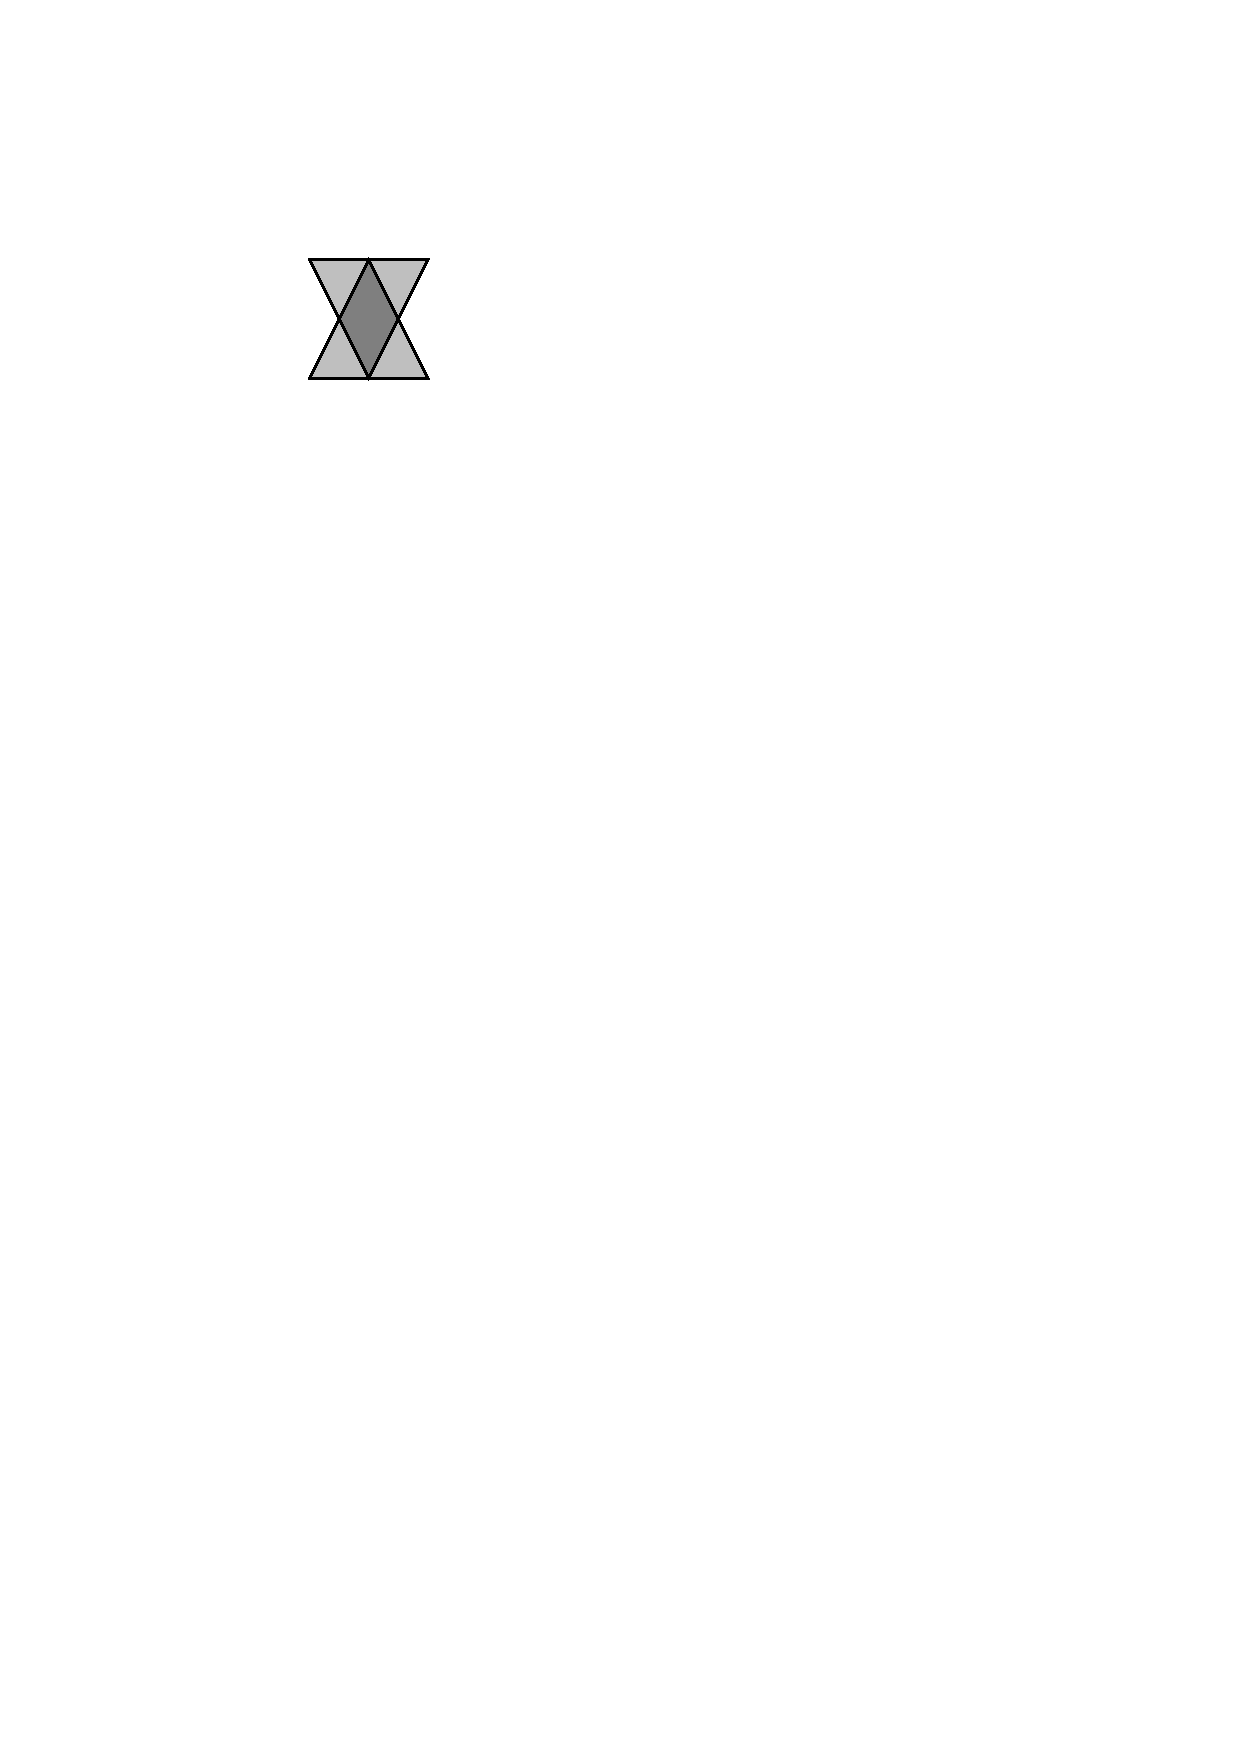
\includegraphics{Boolean_set_operations_2/fig/triangles}
    \end{center}
  \end{minipage}
}

\lcTex{\vspace{-20pt}}
\ccIncludeExampleCode{../examples/Boolean_set_operations_2/ex_do_intersect.C}

% ----------------------------------
\subsection{Polygons with Holes}
\label{bops_ssec:polygons_with_holes}
% ----------------------------------

\begin{figure}[!htp]
\begin{ccTexOnly}
  \begin{center}
  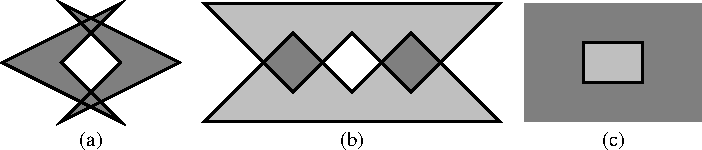
\includegraphics{Boolean_set_operations_2/fig/simple}
  \end{center}
\end{ccTexOnly}
\label{fig:simple}
\begin{ccHtmlOnly}
  <p><center>
    <img src="./fig/simple.gif" border=0 alt="Operations on Strictly
    simple polygons">
  </center>
\end{ccHtmlOnly}
\caption{Operations on strictly simple polygons. (a)~The union of two
polygons, resulting in a point set whose outer boundary is defined by
a simple polygon and contains a polygonal hole in its interior. (b)~The
intersection (darkly shaded) of two polygons (lightly shaded), resulting
in two disjoint polygons. (c)~The complement (darkly shaded) of a strictly
simple polygon (lightly shaded).} 
\end{figure}

In many cases a binary operation that operates on two strictly simple
polygons that have no holes may result in a set of polygon that
contains holes in their interior (see Figure~\ref{fig:simple}~(a)), 
or a set of disjoint polygons (see Figure~\ref{fig:simple}~(b); a similar
set may result from the union, or the symmetric difference, of two disjoint
polygons). Moreover, the complement of a simple polygon is an unbounded set
that contains a hole; see Figure~\ref{fig:simple}~(c).

Regular sets are closed under regularized Boolean set-operations.
These operations accept as input, and may result as output, polygons
with holes. A {\em polygon with holes} represents a point set that may
be bounded or unbounded. In case of a bounded set, its {\em outer
boundary} is represented as a simple (but not necessarily strictly
simple) polygon, whose vertices are oriented in a counterclockwise
order around the interior of the set. In addition, the set may contain
{\em holes}, where each hole is represented as a strictly simple
polygon, whose vertices are oriented in a clockwise order around the
interior of the hole. Note that an unbounded polygon without holes
spans the entire plane. Vertices of holes may coincide with vertices
of the boundary; see below for an example. 

A point set represented by a polygon with holes is considered to be
closed. Therefore, the boundaries of the holes are parts of the set
(and not part of the holes).
The exact definition of the obtained polygon with holes as a result of
a Boolean set-operation or a sequence of such operations is closely
related to the definition of regularized Boolean set-operations, being
the closure of the interior of the corresponding ordinary operation as
explained next.
\newpage
\lcTex{%
  \setlength{\widthRight}{1.4cm}
  \setlength{\widthLeft}{\widthLineReal}
  \addtolength{\widthLeft}{-\widthRight}
  \begin{minipage}{\widthLeft}
}
\label{fig:unique}
\begin{ccHtmlOnly}
  <img src="./fig/unique.gif" border=0 alt="Unique" align=right>
\end{ccHtmlOnly}
Consider, for example, the regular set depicted on the right, which is
the result of the union of three small triangles translated
appropriately. Alternatively, the same set can be reached by taking
the \ccHtmlNoLinksFrom{difference} between a large triangle and a small
upside-down triangle. In general, there are many ways to arrive at 
a particular point set. However, the set of polygons with holes
obtained through the application of any sequence of operations is
unique. The set depicted on the right is represented as a single
polygon having a triangular outer boundary with a single triangluar
hole in its interior --- and not as three triangles that have no holes
at all. As a general rule, if two point sets are connected, then they
belong to the same polygon with holes.
\lcTex{%
  \end{minipage}\hspace{\minipageSpace}
  \begin{minipage}{\widthRight}
    \begin{center}
    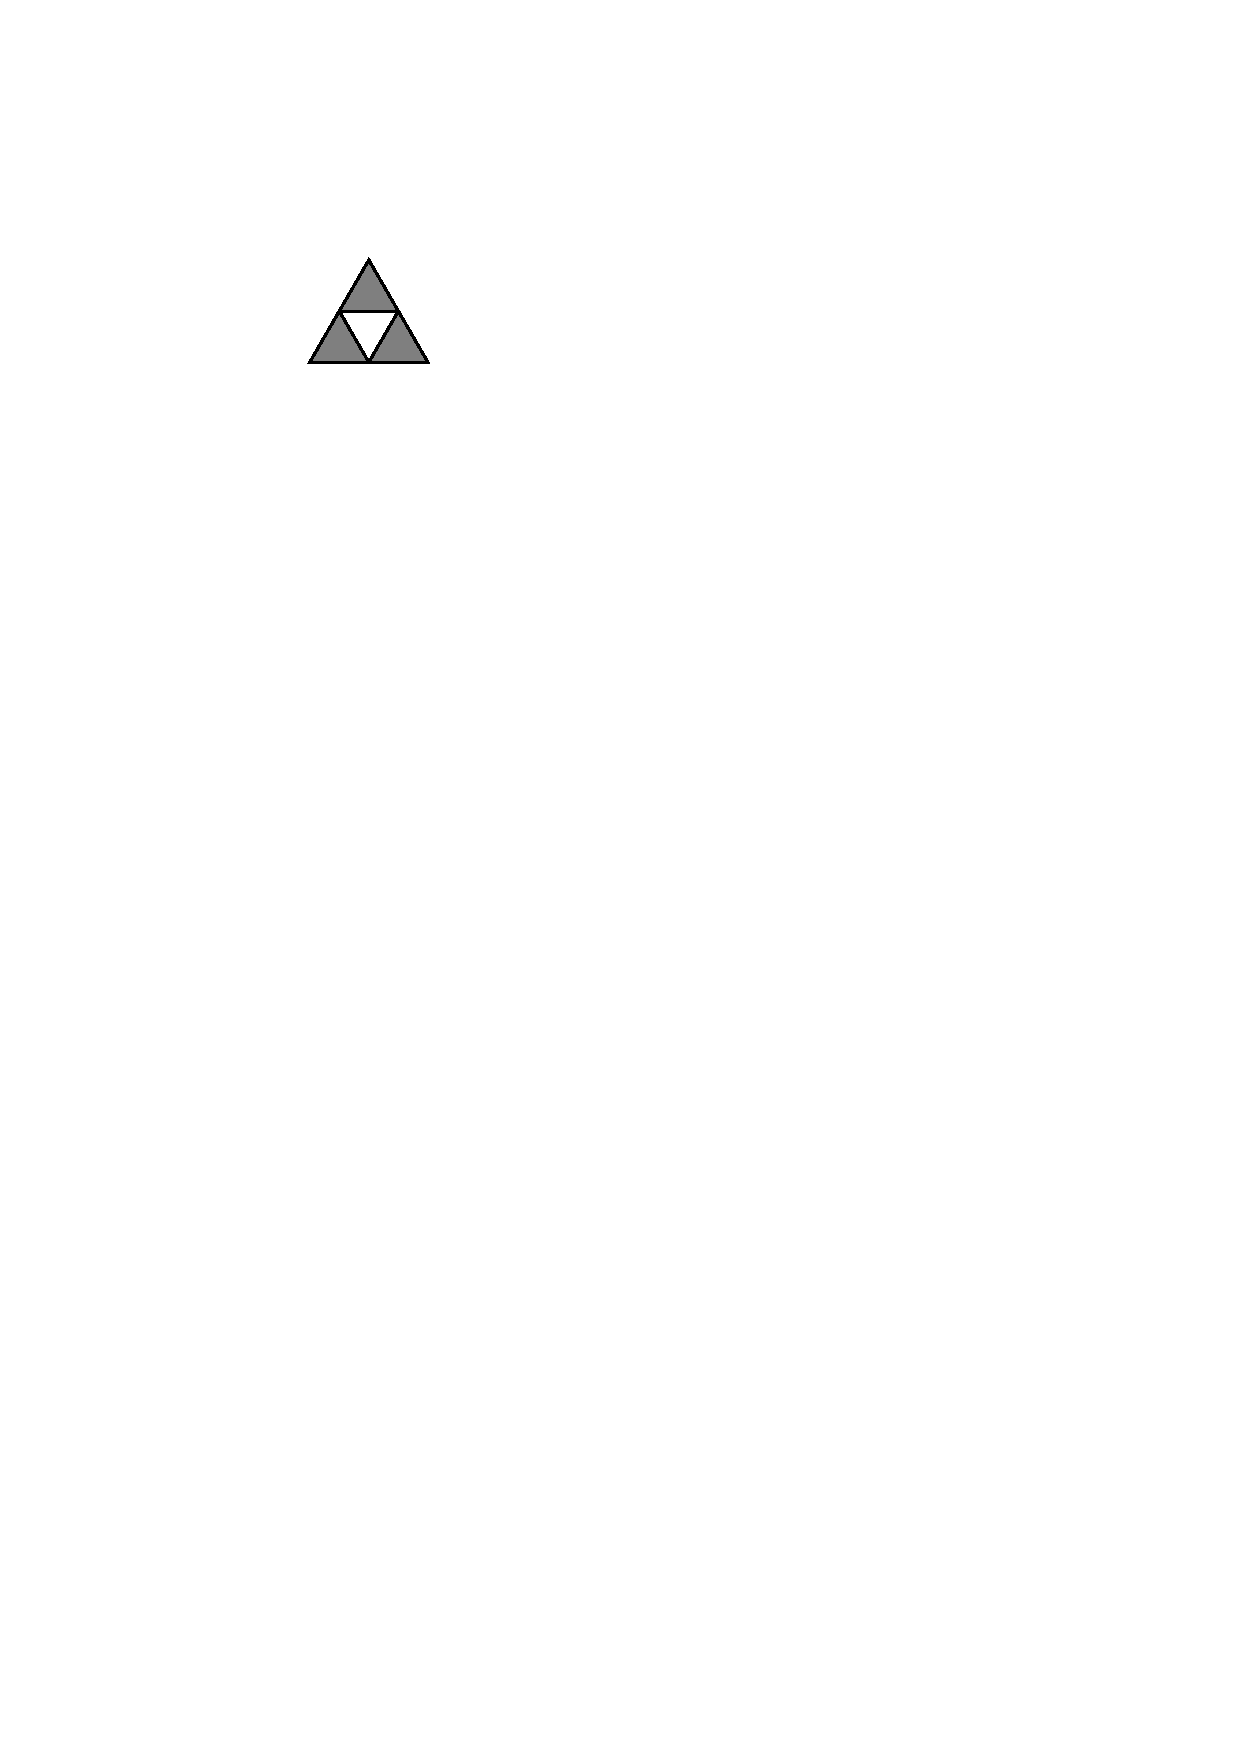
\includegraphics{Boolean_set_operations_2/fig/unique}
    \end{center}
  \end{minipage}
}

The class template \ccc{Polygon_with_holes_2<Kernel,Container>}
represents polygons with holes as described above, where the outer
boundary and the hole boundaries are realized as
\ccc{Polygon_2<Kernel,Container>} objects. Given an instance $P$ of
the \ccc{Polygon_with_holes_2} class, you can use the predicate
\ccc{is_unbounded()} to check whether $P$ is a unbounded set. If it is
bounded, you can obtain the counterclockwise-oriented polygon that
represents its outer boundary through the member function
\ccc{outer_boundary()}. You can also traverse the holes of $P$ through
\ccc{holes_begin()} and \ccc{holes_end()}. The two functions return
iterators of the nested type
\ccc{Polygon_with_holes_2::Hole_const_iterator} that  
defines the valid range of $P$'s holes. The value type of this
iterator is \ccc{Polygon_2}.

The following function demonstrates how to traverse a polygon with holes.
It accepts a \ccc{Polygon_with_holes_2} object and uses the auxiliary
function \ccc{print_polygon()} to prints all its components in a readable
format:
\begin{alltt}
template<class Kernel, class Container>
void print_polygon_with_holes(const CGAL::Polygon_with_holes_2<Kernel, Container> & pwh)
\{
  if (! pwh.is_unbounded()) \{
    std::cout << "\{ Outer boundary = "; 
    print_polygon (pwh.outer_boundary());
  \}
  else
    std::cout << "\{ Unbounded polygon." << std::endl;

  typename CGAL::Polygon_with_holes_2<Kernel,Container>::Holes_const_iterator hit;
  unsigned int k = 1;

  std::cout << "  " << pwh.number_of_holes() << " holes:" << std::endl;
  for (hit = pwh.holes_begin(); hit != pwh.holes_end(); ++hit, ++k) \{
    std::cout << "    Hole #" << k << " = ";
    print_polygon (*hit);
  \}
  std::cout << " \}" << std::endl;
\}
\end{alltt}

The simple versions of the free functions mentioned therefore
accept two \ccc{Polygon_2} object $P$ and $Q$ as their input, while
their output is given using polygon with holes instances:
\begin{itemize}
\item The complement of a simple polygon $P$ is always an unbounded set
with a single polygonal hole. The function \ccc{complement(P)} therefore
returns a polygon-with-holes object that represents the complement of $P$.
\item The union of two polygons $P$ and $Q$ is always a single connected
set, unless of course the two input polygons are completely disjoint. In
the latter case $P \cup Q$ trivially consists of the two input polygons.
The free function \ccc{join(P, Q, R)} therefore returns a Boolean value
indicating whether $P \cap Q \neq \emptyset$. If the two polygons are not
disjoint, it assignes the a polygon with holes object $R$ (which it
accepts by reference) with the union of the regularized union operation
$P \cup Q$.
\item The other three functions, namely \ccc{intersection(P, Q, oi)}, 
\ccc{difference(P, Q, oi)} and \ccc{symmetric_difference(P, Q, oi)}, all
have a similar interface. As the result of these operation may consist
of several disconnected components, they all accept an output iterator
\ccc{oi}, whose value type is \ccc{Polygon_with_holes_2}, and add the
output polygons to its associated container.
\end{itemize}

% ~~~~~~~~~~~~~~~~~~~~~~~~~~~~~~~~~~~~~~~~~~~~~~~~~~~~~~~~~~~~~~~~~~
\subsubsection{Example --- Joining and Intersecting Simple Polygons}
\label{bops_sssec:ex_simple_bops}
% ~~~~~~~~~~~~~~~~~~~~~~~~~~~~~~~~~~~~~~~~~~~~~~~~~~~~~~~~~~~~~~~~~~

The following example demonstartes the usage of the free functions
\ccc{join()} and \ccc{intersect()} for computing the union and the
intersection of the two simple polygons depicted in
Figure~\ref{fig:simple}~(b). The example uses the auxiliary function
\ccc{print_polygon_with_holes()} listed above, which is located in
the header file \ccc{print_utils.h} under the examples folder.

\ccIncludeExampleCode{../examples/Boolean_set_operations_2/ex_simple_join_intersect.C}

% ~~~~~~~~~~~~~~~~~~~~~~~~~~~~~~~~~~~~~~~~~~~~~~~
\subsubsection{Operations on Polygons with Holes}
\label{bops_sssec:pwh_bops}
% ~~~~~~~~~~~~~~~~~~~~~~~~~~~~~~~~~~~~~~~~~~~~~~~

Having introduced polygons with holes and explained how the free functions
output such objects, it is only natural to perform operations on sets that
are represented as polygon with holes, rather than simple polygons.
Indeed, the Boolean set-operations package provides overriden free functions
\ccc{complement()}, \ccc{intersection()}, \ccc{join()}, \ccc{difference()},
\ccc{symmetric_difference()} and \ccc{do_intersect()} that accept
\ccc{General_polygon_with_holes_2} objects as their input. The prototypes of
most functions is the same as of their simpler counterparts that operate
on simple polygons. The only exception is \ccc{complement(P, oi)}, which
outputs a range of polygons with holes that represents the complement
of the polygon with holes $P$.

\lcTex{%
  \setlength{\widthRight}{2.5cm}
  \setlength{\widthLeft}{\widthLineReal}
  \addtolength{\widthLeft}{-\widthRight}
  \begin{minipage}{\widthLeft}
}
\label{fig:sym_diff}
\begin{ccHtmlOnly}
  <img src="./fig/symm_diff.gif" border=0 alt="Unique" align=right>
\end{ccHtmlOnly}
The following example demonstrates how to compute the symmetric
difference between two sets that contain holes. Each set is a
rectangle that contains a rectangular hole in its interior, such that
the symmetric difference between the two sets is a single polygon that
contains of five holes:
\lcTex{%
  \end{minipage}\hspace{\minipageSpace}
  \begin{minipage}{\widthRight}
    \begin{center}
    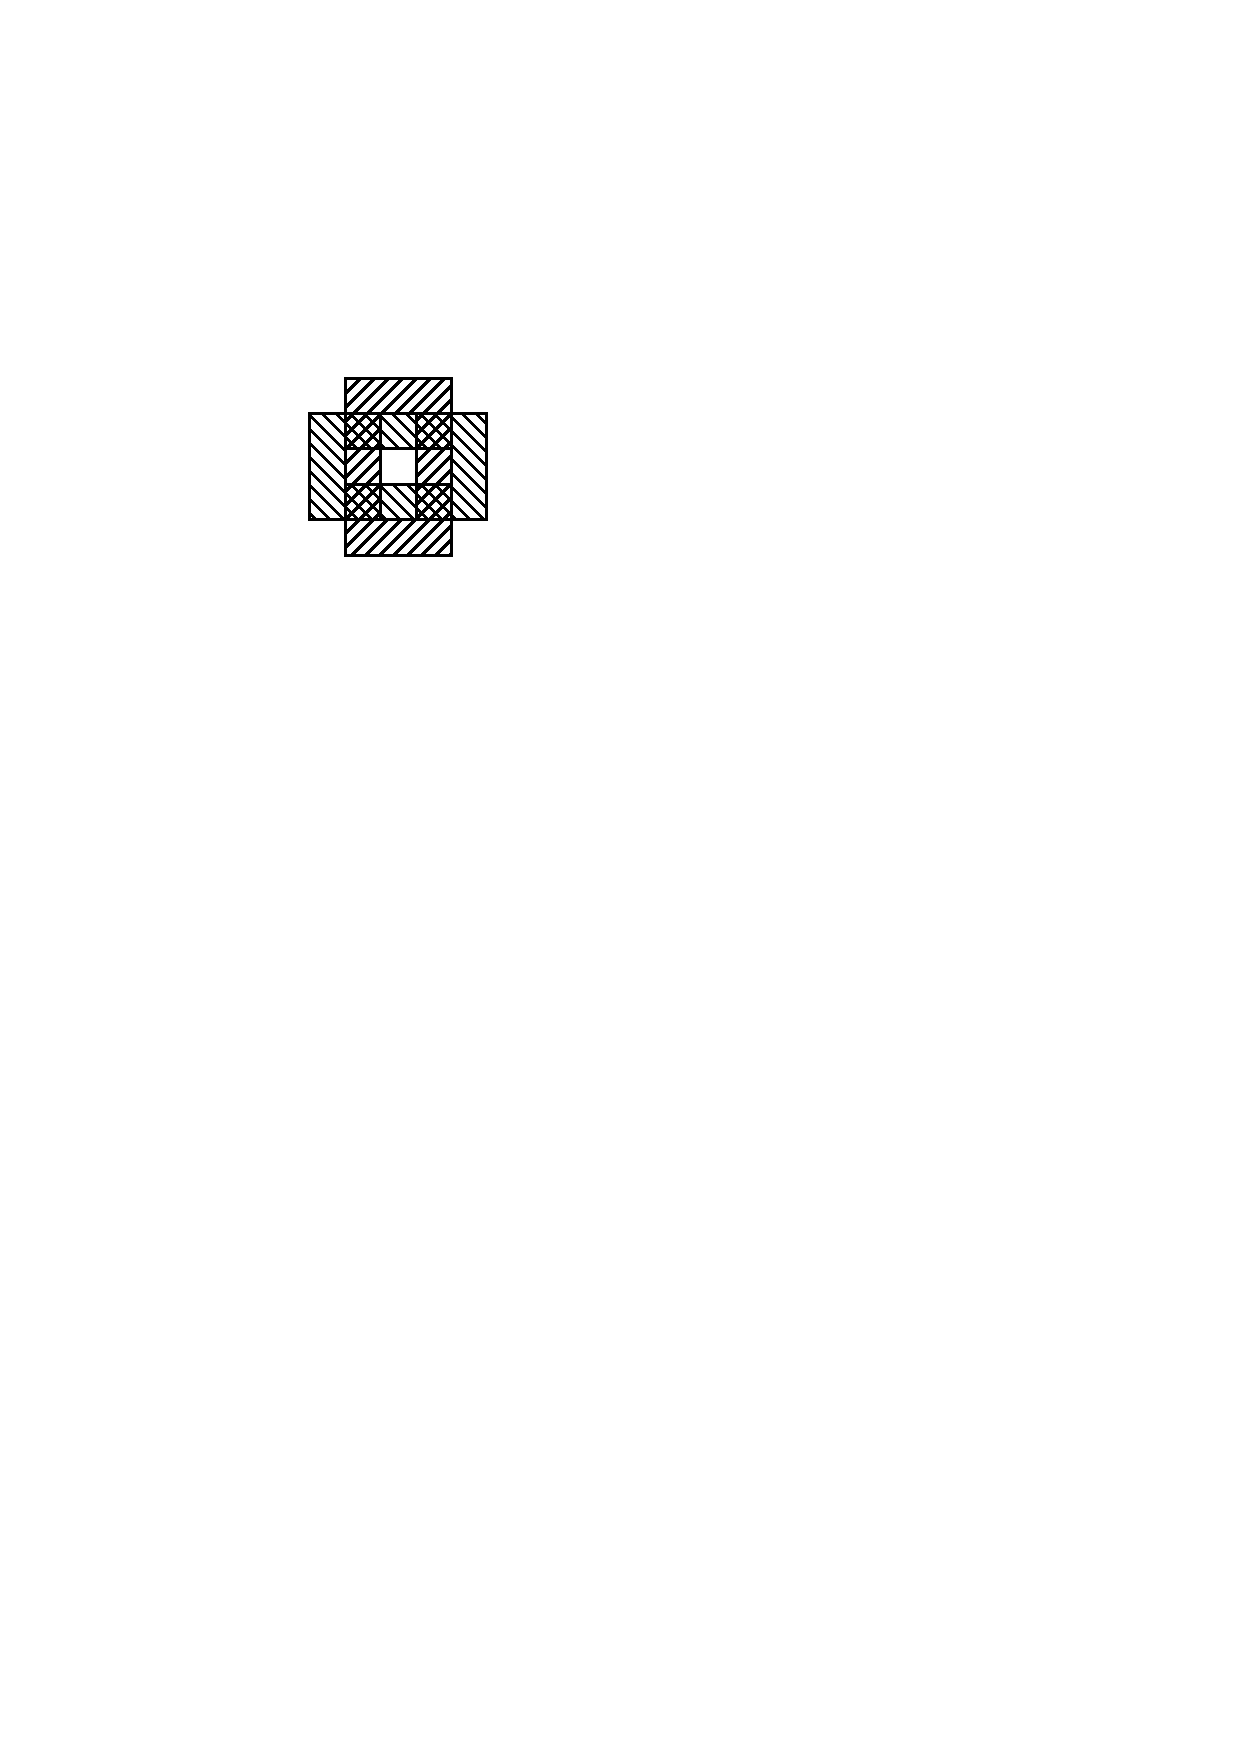
\includegraphics{Boolean_set_operations_2/fig/symm_diff}
    \end{center}
  \end{minipage}
}

\ccIncludeExampleCode{../examples/Boolean_set_operations_2/ex_symmetric_difference.C}

% ------------------------------------
\subsection{Operating on Polygon Sets}
\label{bops_ssec:main_component}
% ------------------------------------

We argue that the result of a regularized operations on two polygons
(or polygons with holes) $P$ and $Q$ is typically a collection of
several disconnected polygons with holes. It is only natural to
represent such a collection in terms of a class, making it possible to
operate on the set resulting from computing, for example, $P \setminus
Q$.

A central component in the Boolean set-operations package is the
\ccc{Polygon_set_2<Kernel, Container>} class-template. An instance of this
class represents a point set formed by the collection of several disconnected
polygons with holes. It employs the \ccc{Arrangement_2} class to represent
this point set in the plane as a planar arrangement; see
Chapter~\ref{chapterArrangement_2}. 

An instance $S$ of a \ccc{Polygon_set_2} class usually represents
the result of a sequence of operations that were applied on some input
polygons. The representation of $S$ is unique, regardless of the particular
sequence of operations that were applied in order to arrive at it.

In addition, a polygon-set object can be constructed from a single
polygon object or from a polygon-with-holes object. Once constructed,
it is possible to insert new polygons (or polygons with holes)
into the set using the \ccc{insert()} method, as long as the inserted
polygons and the existing polygons in the set are disjoint. 
The \ccc{Polygon_set_2} class also provides access functions for
accessing the polygons with holes it contains, and a few queries. The
most improtant query is \ccc{S.oriented_side(q)}, which determined
whether the query point $q$ is contained in the interior of the set
$S$, lies on the boundary of the set, or neither.

The \ccc{General_polygon_set_2} class defines the predicate
\ccc{do_intersect()} and the methods \ccc{complement()}, \ccc{intersection()},
\ccc{join()}, \ccc{difference()} and \ccc{symmetric_difference()} as member
functions. The operands to these functions may be simple polygons 
(\ccc{Polygon_2} object), polygons with holes
(\ccc{General_polygon_with_holes_2} objects), or polygon sets
(\ccc{General_polygon_set_2} objects). Thus, each of the function
mentioned above is actually realized by a set overriding member
functions.

Member functions of the \ccc{General_polygon_set_2} that perform
Boolean set-operations come in two flavors: for example, \ccc{S.join(P, Q)}
computes the union of $P$ and $Q$ and assigned the reuslt to $S$, while
\ccc{S.join(P)} preformes the operation $S \longleftarrow S \cup P$.
Similarly, \ccc{S.complement(P)} sets $S$ to be the complement of $P$,
while $S.complement()$ simply negates the set $S$.

% ~~~~~~~~~~~~~~~~~~~~~~~~~~~~~~~~~~~~~~~~~~
\subsubsection{A Sequence of Set Operations}
\label{bops_sssec:sequence}
% ~~~~~~~~~~~~~~~~~~~~~~~~~~~~~~~~~~~~~~~~~~

The free functions reviewed in Section~\ref{bops_ssec:polygons_with_holes}
serve as a wrapper for the polygon-set class, and are only provided for
convinience. A typical such function constructs a pair of
\ccc{General_polygon_set_2} objects, invokes the appropriate method to
apply the desired Boolean operation, and transforms the resulting
polygon set to the required output format. Thus, when several
operations are performed in a sequence, it is much more efficient to
use the member functions of the \ccc{General_polygon_set_2} type
directly, as the extraction of the polygons from the internal
representation for some operation, and the reconstruction of the
internal representation for the succeeding operation could be time
consuming.

\lcTex{%
  \setlength{\widthRight}{2.3cm}
  \setlength{\widthLeft}{\widthLineReal}
  \addtolength{\widthLeft}{-\widthRight}
  \begin{minipage}{\widthLeft}
}
\label{fig:sequence}
\begin{ccHtmlOnly}
  <p><center>
    <img src="./fig/sequence.gif" border=0 alt="A sequence of operation" align=right>
  </center>
\end{ccHtmlOnly}
The next example performs a sequence of three Boolean set-operations.
First, it computes the union of two simple polygons depicted in
Figure~\ref{fig:simple}~(a). It then computes the complement of the result
of the union operation. Finally, it computes the intersection of the result
of the complement operation with a rectangle, confining the final result to 
the area of the rectangle. The resulting set $S$ is comprised of two
components: a polygon with a hole, and a simple polygon contained in the
interior of this hole.
\lcTex{%
  \end{minipage}\hspace{\minipageSpace}
  \begin{minipage}{\widthRight}
    \begin{center}
    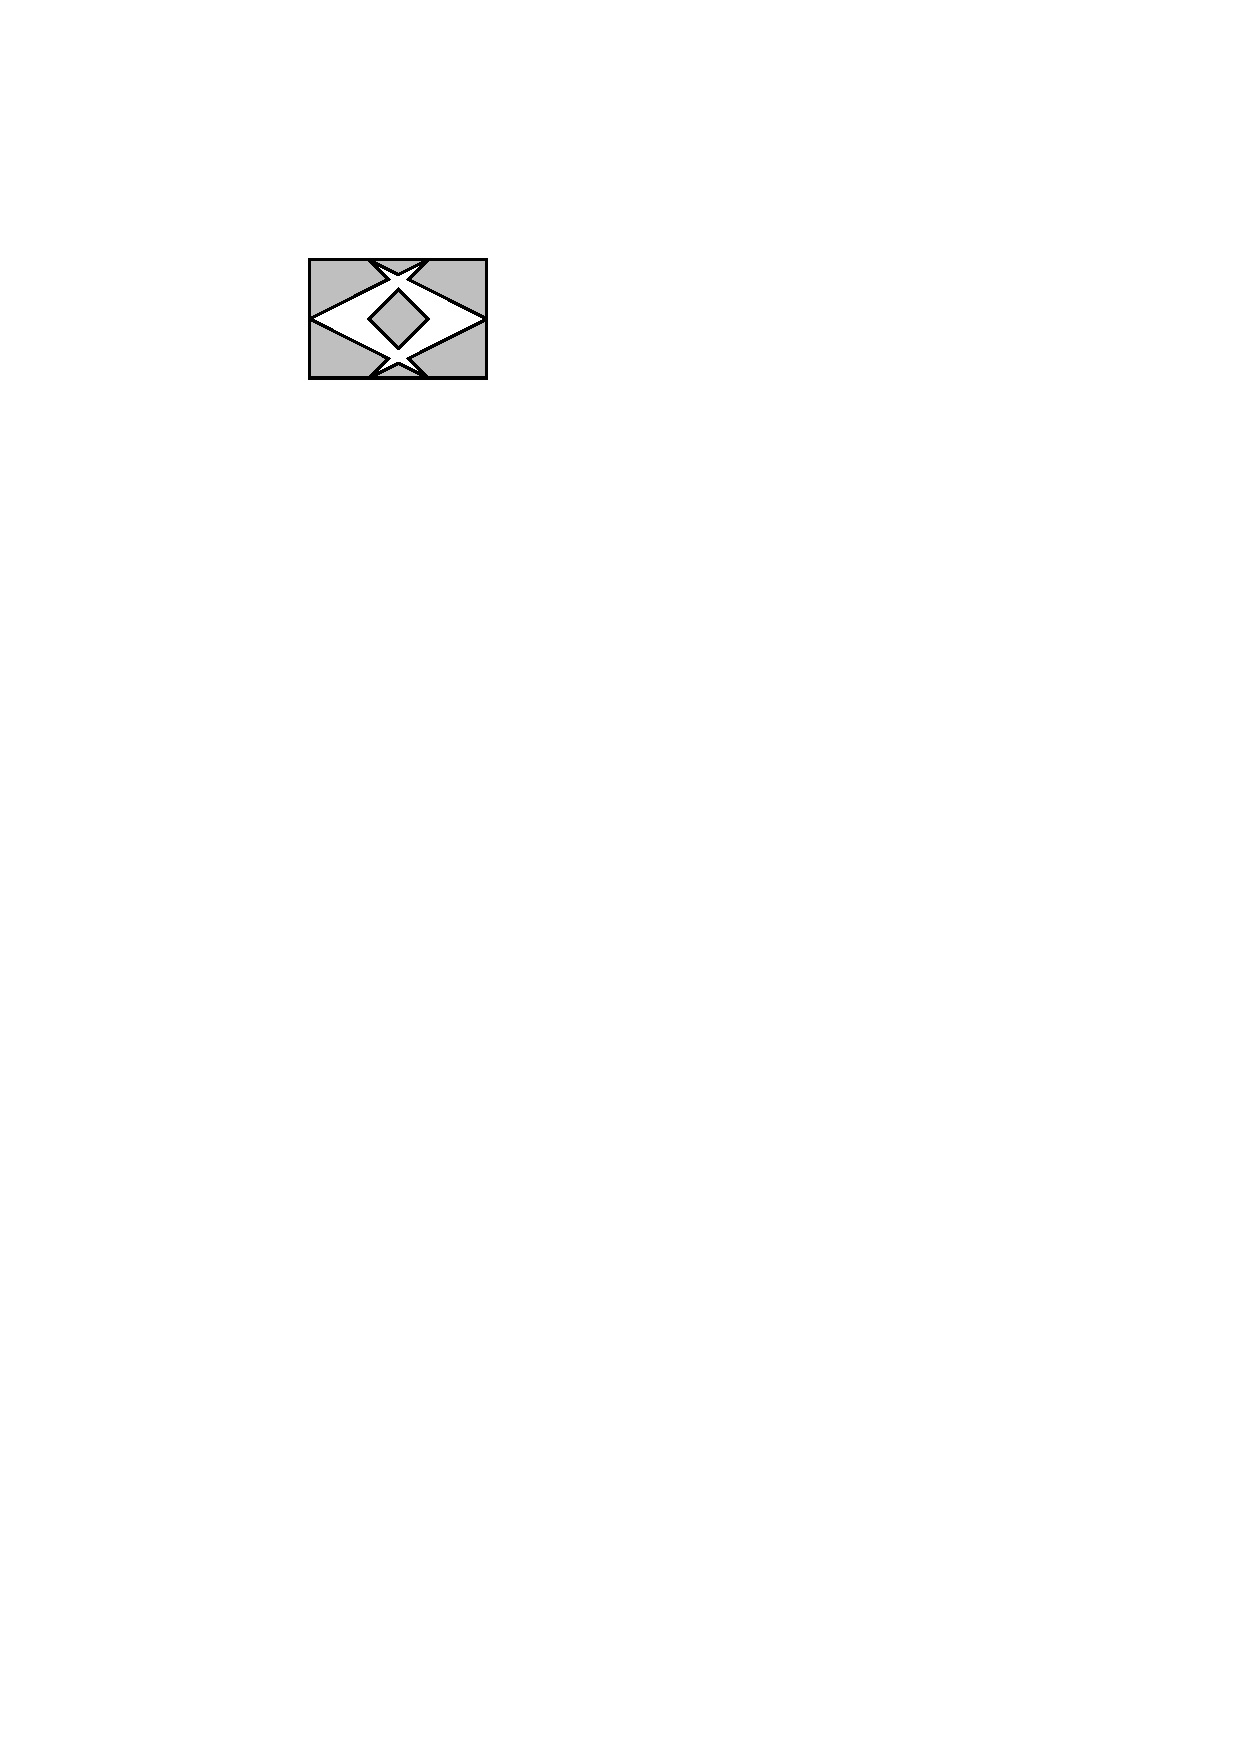
\includegraphics{Boolean_set_operations_2/fig/sequence}
    \end{center}
  \end{minipage}
  \vspace{2pt}
}

\ccIncludeExampleCode{../examples/Boolean_set_operations_2/ex_sequence.C}

% ~~~~~~~~~~~~~~~~~~~~~~~~~~~~~~~~~~~~~~~~~~~~~~~~~
\subsubsection{Inserting Non Intersecting Polygons}
\label{bops_ssec:insert_ni}
% ~~~~~~~~~~~~~~~~~~~~~~~~~~~~~~~~~~~~~~~~~~~~~~~~~

If you want to compute the union of a polygon $P$ ($P$ may be a simple
polygon or a polygon-with-holes object) with a general-polygon set
$R$, and store the result in $R$, you can construct a polygon set
$S(P)$, and apply the {\em union} operation as follows:
\begin{alltt}
  General_polygon_2 S (P);
  R.join (S);
\end{alltt}

As a matter of fact, you can apply the union operation directly:
\begin{alltt}
  R.join (P);
\end{alltt}

However, if you know that the polygon does not intersect any one of the
polygons represented by $R$, you can use the more efficient method
\ccc{insert()}:
\begin{alltt}
  R.insert (P);
\end{alltt}

As \ccc{insert()} assumes that $P \cap R = \emptyset$, it does try to
compute intersections between the boundaries of $P$ and of $R$. This
fact significantly speeds up the insertion process in comparison with the
insertion of a non-disjoint polygon that intersects $R$.

The \ccc{join()} function is also overloaded, so it can also accept a
range of polygons. When a range of polygons are inserted into a
polygon set $S$, all the general polygons in the range and the general
polygons represented by $S$ must be pairwise disjoint in their interiors.

% -------------------------------------------
\subsection{Performing Aggregated Operations}
\label{bops_ssec:agg_ops}
% -------------------------------------------

There are a few options to compute the union of a set of polygons
$P_1, \ldots P_m$. You can do it incrementally as follows. At each step
compute the union of $S_{k-1} = \bigcup_{i=1}^{k-1}{P_i}$ 
with $P_{k}$ and obtain $S_k$. Namely, if the polygon set is given
as a pair of iterator \ccc{[begin, end)}, the following loop computes
their union in $S$.
\begin{alltt}
  InputIterator iter = begin;
  Polygon_set_2 S (*iter);

  while (++iter != end) \{
    S.join (*iter);
    ++iter;
  \}
\end{alltt}  
A second option is to use a divide-and-conquer approach. You bisect
the set of polygons into two sets. Compute the union of each set
recursively and obtain the partial results in $S_1$ and $S_2$, and
finally, you compute the union $S_1 \cup S_2$. However, the union
operation can be done more efficiently for sparse polygons, having
a relatively small number of intersections, using a third option that
simultaneously computes the union of all polygons. This is done by 
constructing a planar arrangement of all input polygons, utilizing the
sweep-line algorithm, then extracting the result from the
arrangement. Similarly, it is also possible to aggregately compute the
intersection $\bigcap_{i=1}^{m}{P_i}$ of a set of input polygons.

Our package provides the free overloaded functions \ccc{join()} and
\ccc{intersect()} that aggregately compute the union and the intersection
of a range of input polygons. There is no restriction on the polygons in the
range --- naturally, they may intersect each other.
The package provides the overloaded free function 
\ccc{do_intersect(begin, end)} that determines whether the polygons in the
range defined by the two input iterators \ccc{[begin, end)} intersect.

The class \ccc{General_polygon_set_2} also provides equivalent member
functions that aggragately operate on a range of input polygons or
polygons with holes. When such a member function is called, the general 
polygons represented by the current object are considered operands as 
well. Thus, you can easily compute the union of our polygon range as
follows:
\begin{alltt}
  Polygon_set_2 S;
  S.join (begin, end);
\end{alltt} 

% RWRW : A separate section about Circular_polygon_2<Kernel> ?

% ==================================================
\section{Boolean Set-Operations on General Polygons}
\label{bops_sec:bops_gen}
% ==================================================

\lcTex{%
  \setlength{\widthRight}{1.4cm}
  \setlength{\widthLeft}{\widthLineReal}
  \addtolength{\widthLeft}{-\widthRight}
  \begin{minipage}{\widthLeft}
}
\label{fig:general_polygon}
\begin{ccHtmlOnly}
  <p><center>
    <img src="./fig/general_polygon.gif" border=0 alt="A general polygon" align=right>
  </center>
\end{ccHtmlOnly}
In previous sections ordinary polygons were dealt with. Namely, closed
point sets bounded by piecewise linear curves. The Boolean
set-operations package allows a more general geometric mapping of the
polygon edges. The operations provided by the package operate on point
sets bounded by $x$-monotone segments of general curves (e.g., conic
arcs and segments of polynomial functions). For example, the point set
depicted on the right is general polygon bounded by two $x$-monotone
circular arcs that correspond to the lower half and the upper half of
a circle.
\lcTex{%
  \end{minipage}\hspace{\minipageSpace}
  \begin{minipage}{\widthRight}
    \begin{center}
    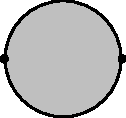
\includegraphics{Boolean_set_operations_2/fig/general_polygon}
    \end{center}
%    A general polygon.
  \end{minipage}
  \vspace{2pt}
}

Using the topological terminology, a general polygon can represent any
simply-connected point set whose boundary is a strictly simple curve.
Such a polygon is a model of the \ccc{GeneralPolygon_2} concept. A model
of this concept must fulfill the following requirements:
\begin{itemize}
\item A general polygon is constructible from a range of pairwise
interior disjoint $x$-monotone curves $c_1, \ldots, c_n$. The target
point of the $k$th curve $c_k$ and the source point of the next curve
in the range (in a cyclic order) must coincide, such that this point
defines the $k$th polygon vertex. 
\item It is possible to traverse the $x$-monotone curves that form the
edges of a general polygon.
\end{itemize}

\lcTex{%
  \setlength{\widthRight}{1.4cm}
  \setlength{\widthLeft}{\widthLineReal}
  \addtolength{\widthLeft}{-\widthRight}
  \begin{minipage}{\widthLeft}
}
\label{fig:general_polygon_with_holes}
\begin{ccHtmlOnly}
  <p><center>
    <img src="./fig/general_polygon_with_holes.gif" border=0 alt="A general polygon with holes" align=right>
  </center>
\end{ccHtmlOnly}
The concept \ccc{GeneralPolygonWithHoles_2} is defined in an analogous
way to the definition of linear polygons with holes. A model of this
concept represent a bounded or an unbounded set that may not be simply
connected, and must provide the following operations:
\lcTex{%
  \end{minipage}\hspace{\minipageSpace}
  \begin{minipage}{\widthRight}
    \begin{center}
    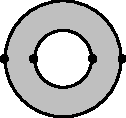
\includegraphics{Boolean_set_operations_2/fig/general_polygon_with_holes}
    \end{center}
%    A general polygon with holes.
  \end{minipage}
  \vspace{1pt}
}
\begin{itemize}
\item Construction for a general polygon that represent the outer boundary
and a range of general polygons that represent the holes.
\item Accessing the general polygons that represents the outer boundary
(in case of a bounded set).
\item Traversing the holes.
\end{itemize}
In Section~\ref{bops_sec:bops_lin} we introduced the classes
\ccc{Polygon_2} and \ccc{Polygon_with_holes_2} that model the concepts
\ccc{GeneralPolygon_2} and \ccc{GeneralPolygonWithHoles_2}
respectively. In this section we introduce other models of these two
concepts.

The central class-template \ccc{General_polygon_set_2<Traits>} is used to
represent point sets that are comprised of a finite number of general
polygons with holes that are pairwise disjoint, and provides various Boolean
set-operations on such sets. It is parameterized by a {\em traits}
class that defines the type of points used to represent polygon
vertices and the type of $x$-monotone curves that represent the
polygon edges. The traits class also provides primitive geometric
operations that operate on objects of these types. An instatiated
\ccc{General_polygon_set_2} class defines the nested types 
\ccc{General_polygon_set_2<Traits>::Polygon_2} and
\ccc{General_polygon_set_2<Traits>::Polygon_with_holes_2}, which model
the concept \ccc{GeneralPolygon_2} concept and
\ccc{GeneralPolygonWithHoles_2} respectively.

% ------------------------------------
\subsection{The Traits-Class Concepts}
\label{bops_ssec:traits_concepts}
% ------------------------------------

The traits class used to instantiate the \ccc{General_polygon_set_2}
class template must model the concept \ccc{GeneralPolygonSetTraits_2},
and is tailored to handle a specific family of curves. The concept
\ccc{GeneralPolygonSetTraits_2} refines the concept
\ccc{ArrangementDirectionalXMonotoneTraits} specified next.

The concept \ccc{ArrangementDirectionalXMonotoneTraits} refines the 
concept \ccc{ArrangementXMonotoneTraits_2} (see 
Section~\ref{arr_sssec:insert_x_mon} in the 2D Arrangements chapter).
Thus, a model of this concept must define the type \ccc{X_monotone_curve_2}, 
which represents an $x$-monotone curve, and the type \ccc{Point_2}, 
with represents a planar point. Such a point may be an endpoint of an
$x$-monotone curve or an intersection point between two curves.
It must also provide various geometric predicates and operations 
on these types listed by the base concept, such as determining whether
a point lies above or below an $x$-monotone curve, computing the
intersections between two curves, etc. Note that the base concept does
not assume that $x$-monotone curves are directed: an $x$-monotone
curve is not required to have a designated {\em source} and {\em
target}, it is only required to determine the left (lexicographically
smaller) and the right (lexicographically larger) endpoints of a given
curve.

The \ccc{ArrangementDirectionalXMonotoneTraits} concept treats its
$x$-monotone curves as directed objects. It thus requires two additional
operations on $x$-monotone curves:
\begin{itemize}
\item Given an $x$-monotone curve, compare its source and target points
lexicographically.
\item Given an $x$-monotone curve, construct its opposite curve (namely,
swap its source and target points).
\end{itemize}

The traits classes \ccc{Arr_segment_traits_2}, 
\ccc{Arr_non_caching_segment_traits}, \ccc{Arr_circle_segment_traits_2},
\ccc{Arr_conic_traits_2} and \ccc{Arr_rational_arc_traits_2}, which are 
bundeled in the \ccc{Arrangement_2} package and distributed with \cgal,
are all models of the refined concept 
\ccc{ArrangementDirectionalXMonotoneTraits}.\footnote{The
\ccc{Arr_polyline_traits_2} class is {\em not} a model of the, 
\ccc{ArrangementDirectionalXMonotoneTraits} concept, as the
$x$-monotone curve it defines is always directed from left to
right. Thus, an opposite curve cannot be constructed. However, it is
not very useful to construct a polygon whose edges are polylines, as
an ordinary polygon with linear edges can represent the same entity.}

Just as with the case of computations using models of the 
\ccc{ArrangementXMonotoneTraits_2} concept, operations are robust only
when exact arithmetic is used. When inexact arithmetic is used,
(nearly) degenerate configurations may result in abnormal termination
of the program or even incorrect results.

% ---------------------------------------------------
\subsection{Operating on Polygons with Circular Arcs}
\label{bso_ssec:circ_seg}
% ---------------------------------------------------

Two traits classes are distributed with \cgal. The first one is named
\ccc{Gps_segment_traits_2}, and it is used to perform Boolean
set-operations on oridnary polygons and polygons with holes. In fact,
the class \ccc{Polygon_set_2} introduced in
Section~\ref{bops_ssec:main_component} is a specialization of
\ccc{General_polygon_set_2<Gps_segment_traits_2>}. This class defined
its polygon and polygon with holes types, such that the usage of this
traits class is encapsulated in the polygon-set class.

The other predefined traits class is named 
\ccc{Gps_circle_segment_traits_2<Kernel>} and is parameterized by a
geometric \cgal\ kernel. By instantiating the \ccc{General_polygon_set_2}
with this traits class, we obtain the representation of a polygon whose
boundary may be comprised of line segments and circular arcs.
The circle--segment traits class provides predicates and constructions
on non-linear objects; yet, it uses only rational arithmetic and is
very efficient as a consequence.

\lcTex{%
  \setlength{\widthRight}{2.4cm}
  \setlength{\widthLeft}{\widthLineReal}
  \addtolength{\widthLeft}{-\widthRight}
  \begin{minipage}{\widthLeft}
}
\label{fig:circle_recs}
\begin{ccHtmlOnly}
  <p><center>
    <img src="./fig/circles_rects.gif" border=0 alt="Union of circles
    and rectangles" align=right>
  </center>
\end{ccHtmlOnly}
The following example uses the \ccc{Gps_circle_segment_traits_2} class
to compute the union of four rectangles and four circles. Each circle
is represented as a general polygon having two $x$-monotone circular arcs.
The union is computed incrementally, resulting with a single polygon with
a single hole, as depicted on the right. Note that as the four circles
are disjoint, their union is computed with the \ccc{insert} method,
while the union with the rectangles is computed with the \ccc{join}
operator.
\lcTex{%
  \end{minipage}\hspace{\minipageSpace}
  \begin{minipage}{\widthRight}
    \begin{center}
    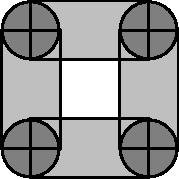
\includegraphics{Boolean_set_operations_2/fig/circles_rects}
    \end{center}
%    A general polygon with holes.
  \end{minipage}
  \vspace{2pt}
}

\ccIncludeExampleCode{../examples/Boolean_set_operations_2/ex_circle_segment.C}

% ---------------------------------------------
\subsection{General Polygon Set Traits Adapter}
\label{bso_ssec:general_polygon_concept}
% ---------------------------------------------

The concept \ccc{GeneralPolygon_2} and its generic model 
\ccc{General_polygon_2<ArrDirectionalXMonotoneTraits>} facilitate the 
production of general-polygon set traits classes. A model of the concept 
\ccc{GeneralPolygon_2} represents a simple point-set in the plane bounded 
by $x$-monotone curves. As opposed to the plain \ccc{Traits::Polygon_2} type 
defined by any traits class, it must define the type 
\ccc{X_monotone_curve_2}, which represents an $x$-monotone curve of the 
point-set boundary. It must provide a constructor from a range of such 
curves, and a pair of methods, namely \ccc{curves_begin()} and 
\ccc{curves_end()}, that can be used to iterate over the point-set boundary 
curves.
 
The class-template \ccc{General_polygon_2<ArrDirectionalXMonotoneTraits>}
models the concept \ccc{GeneralPolygon_2}. Its template parameter must be
instantiated with a model of the concept
\ccc{ArrangementDirectionalXMonotoneTraits_2} from which it obtains the 
\ccc{X_monotone_curve_2} type, and it uses the necessary 
operations on this type provided by such a model to maintain a container 
of directed curves of type \ccc{X_monotone_curve_2}, which represents the 
boundary of the general polygon.

The class-template 
\ccc{Gps_traits_2<ArrDirectionalXMonotoneTraits,GeneralPolygon>}
models the concept \ccc{GeneralPolygonSetTraits_2}. Its implementation is 
rather simple, as it is derived from the instantiated template-parameter 
\ccc{ArrXMonotoneTraits} inheriting its necessary types and methods, 
and it exploits the methods provided by the instantiated parameter 
\ccc{GeneralPolygon} --- a model of the concept \ccc{GeneralPolygon_2}.
By default, the \ccc{GeneralPolygon} parameter is defined as
\ccc{General_polygon_2<ArrangementDirectionalXMonotoneTraits_2>}

The code excerpt listed below defines a general-polygon set type that
can be used to perform Boolean set-operations on point sets bounded by
linear segments used by the \ccc{Arrangement_2} class by default. A
model of the \ccc{GeneralPolygon_2} concept that represents a
(linear) polygon bounded by curves of type \ccc{Arr_segment_2} is
generated. The later is obtained from the instantiated parameter
\ccc{Arr_segment_traits_2}, which defines \ccc{Arr_segment_2} to be
its exposed type \ccc{X_monotone_curve_2}.
\begin{alltt}
typedef CGAL::Gmpq                              	   Number_type;
typedef CGAL::Cartesian<Number_type>            	   Kernel;
typedef CGAL::Arr_segment_traits_2<Kernel>      	   Arr_traits_2;
typedef CGAL::General_polygon_2<Arr_traits_2>   	   General_polygon_2;
typedef CGAL::Gps_traits_2<Arr_traits_2,General_polygon_2> Traits_2;
typedef CGAL::General_polygon_set_2<Traits_2>              General_polygon_set_2;
\end{alltt}

\lcTex{%
  \setlength{\widthRight}{6cm}
  \setlength{\widthLeft}{\widthLineReal}
  \addtolength{\widthLeft}{-\widthRight}
  \begin{minipage}{\widthLeft}
}
\label{fig:conics}
\begin{ccHtmlOnly}
  <p><center>
    <img src="./fig/conic_arcs.gif" border=0 alt="Conic arcs" align=right>
  </center>
\end{ccHtmlOnly}
Swapping the linear arrangement-traits \ccc{Arr_segment_traits_2}
above with a traits class that handle conic arcs, such as
\ccc{Arr_conic_traits_2}, results with the definition of a
general-polygon set type that can be used to perform Boolean 
set-operations on point sets bounded by conic arcs of type
\ccc{Arr_conic_2}. The next example computes the intersection of the
two general polygons depicted on the right. One is an ellipse
given by $x^2 + 9y^2 - 9 = 0$, and the other is bounded by the two
parabolic arcs whose underlying parabola are given by 
$x^2 + 2y - 4 = 0$, and $x^2 - 2y - 4 = 0$. The code in the example adapts
the traits model that handles conics included with the \ccc{Arrangement_2}
package.
\lcTex{%
  \end{minipage}\hspace{\minipageSpace}
  \begin{minipage}{\widthRight}
    \begin{center}
    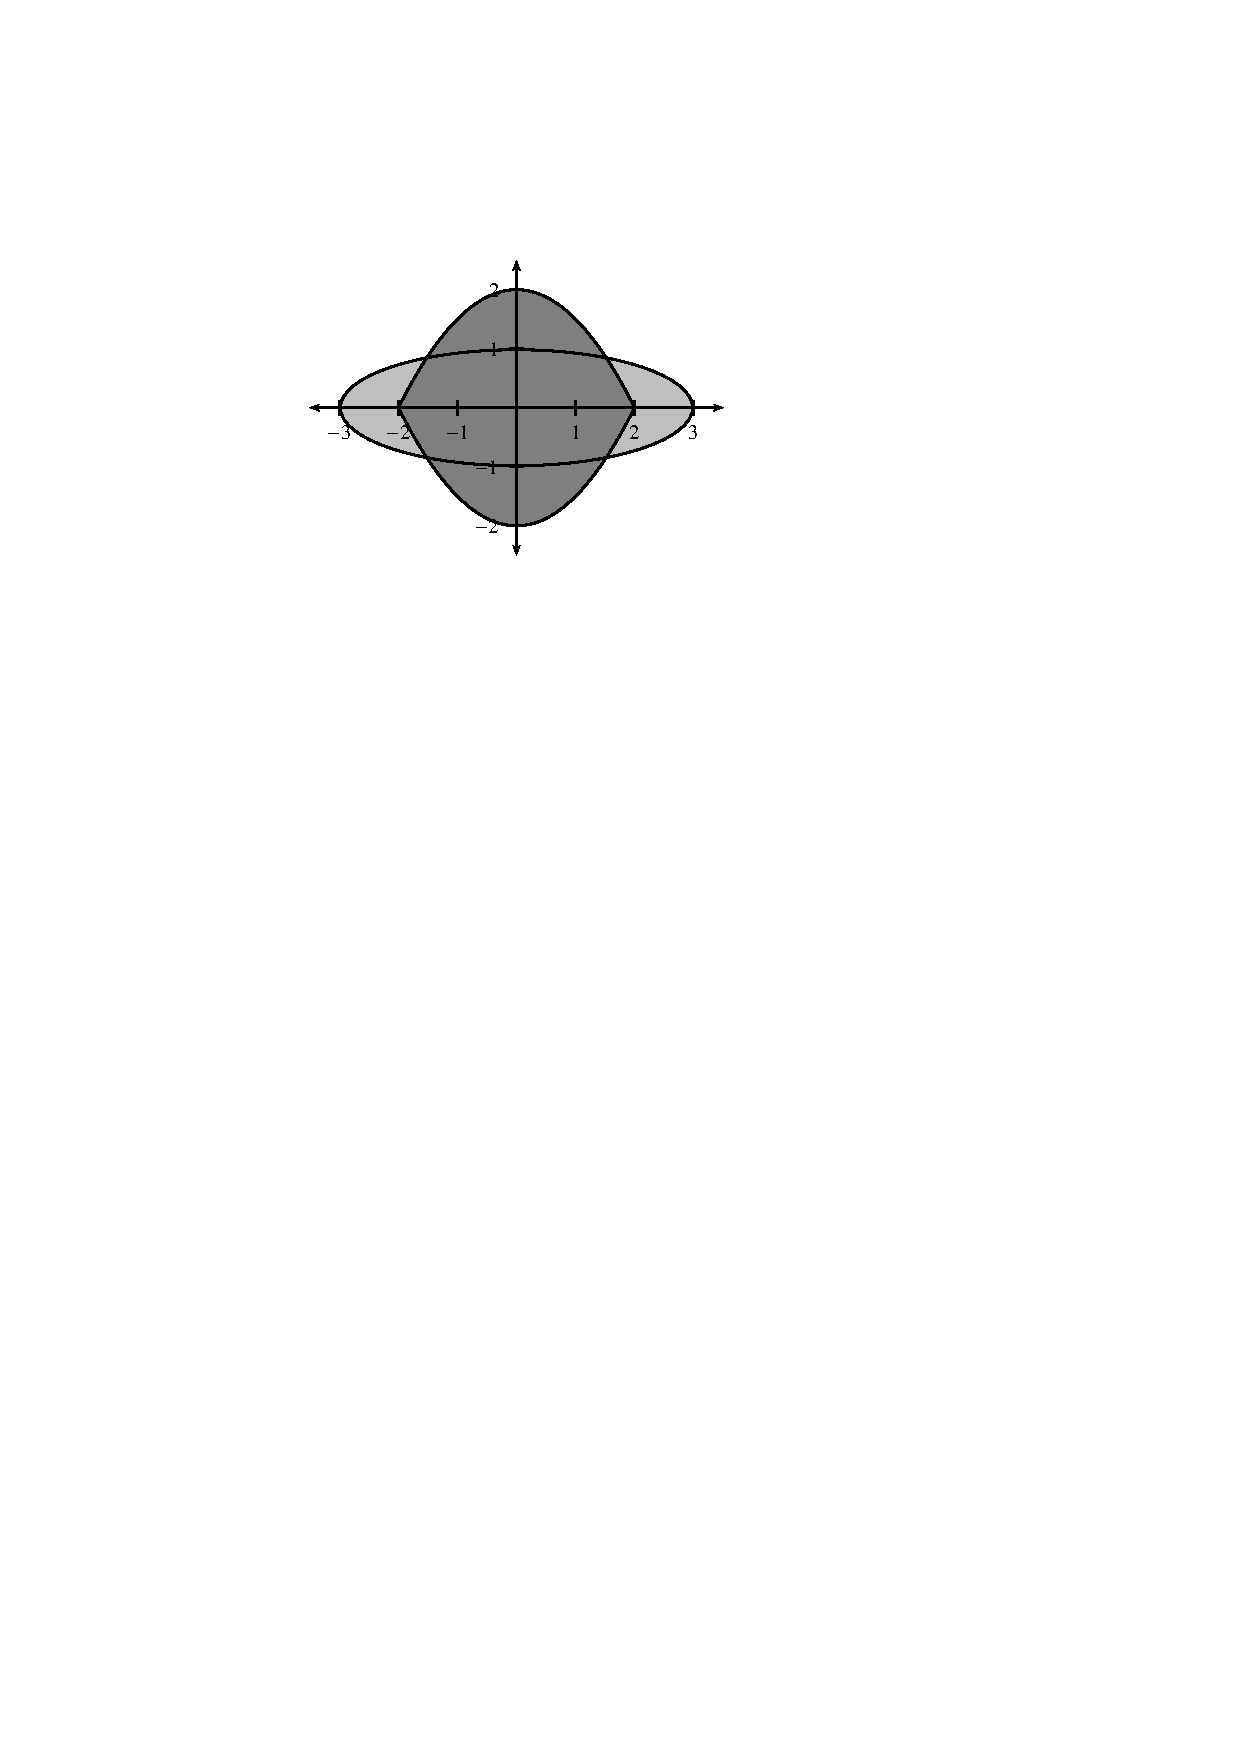
\includegraphics{Boolean_set_operations_2/fig/conic_arcs}
% Conic arcs.
    \end{center}
  \end{minipage}
}

\ccIncludeExampleCode{../examples/Boolean_set_operations_2/ex_traits_adapter.C}

% ------------------------------------------
\subsection{Example - Aggregated Operations}
\label{bops_ssec:aggregated_gen_ops}
% ------------------------------------------

In Section~\ref{bops_ssec:agg_ops} we describe how aggragated union
and intersection operations can be applied to a collection of ordinary
polygons or polygons with holes. Naturally, the aggregated operations
can be applied also to collections of general polygons. As was the
case with ordinary polygons, using aggregated operations is
recommended when the number of intersections of the input polygons
is of the same order of magnitude as the complexity of the result. If
this is not the case, computing the result incrementally may prove
faster.

\lcTex{%
  \setlength{\widthRight}{3.4cm}
  \setlength{\widthLeft}{\widthLineReal}
  \addtolength{\widthLeft}{-\widthRight}
  \begin{minipage}{\widthLeft}
}
\label{fig:disks}
\begin{ccHtmlOnly}
  <p><center>
    <img src="./fig/disks.gif" border=0 alt="Union of disks" align=right>
  </center>
\end{ccHtmlOnly}
The next example computes the union of eight unit discs whose centers are
placed a unit distance from the origin, as depicted to the right. The example
also allows users to provide a different number of discs through the command
line.
\lcTex{%
  \end{minipage}\hspace{\minipageSpace}
  \begin{minipage}{\widthRight}
    \begin{center}
    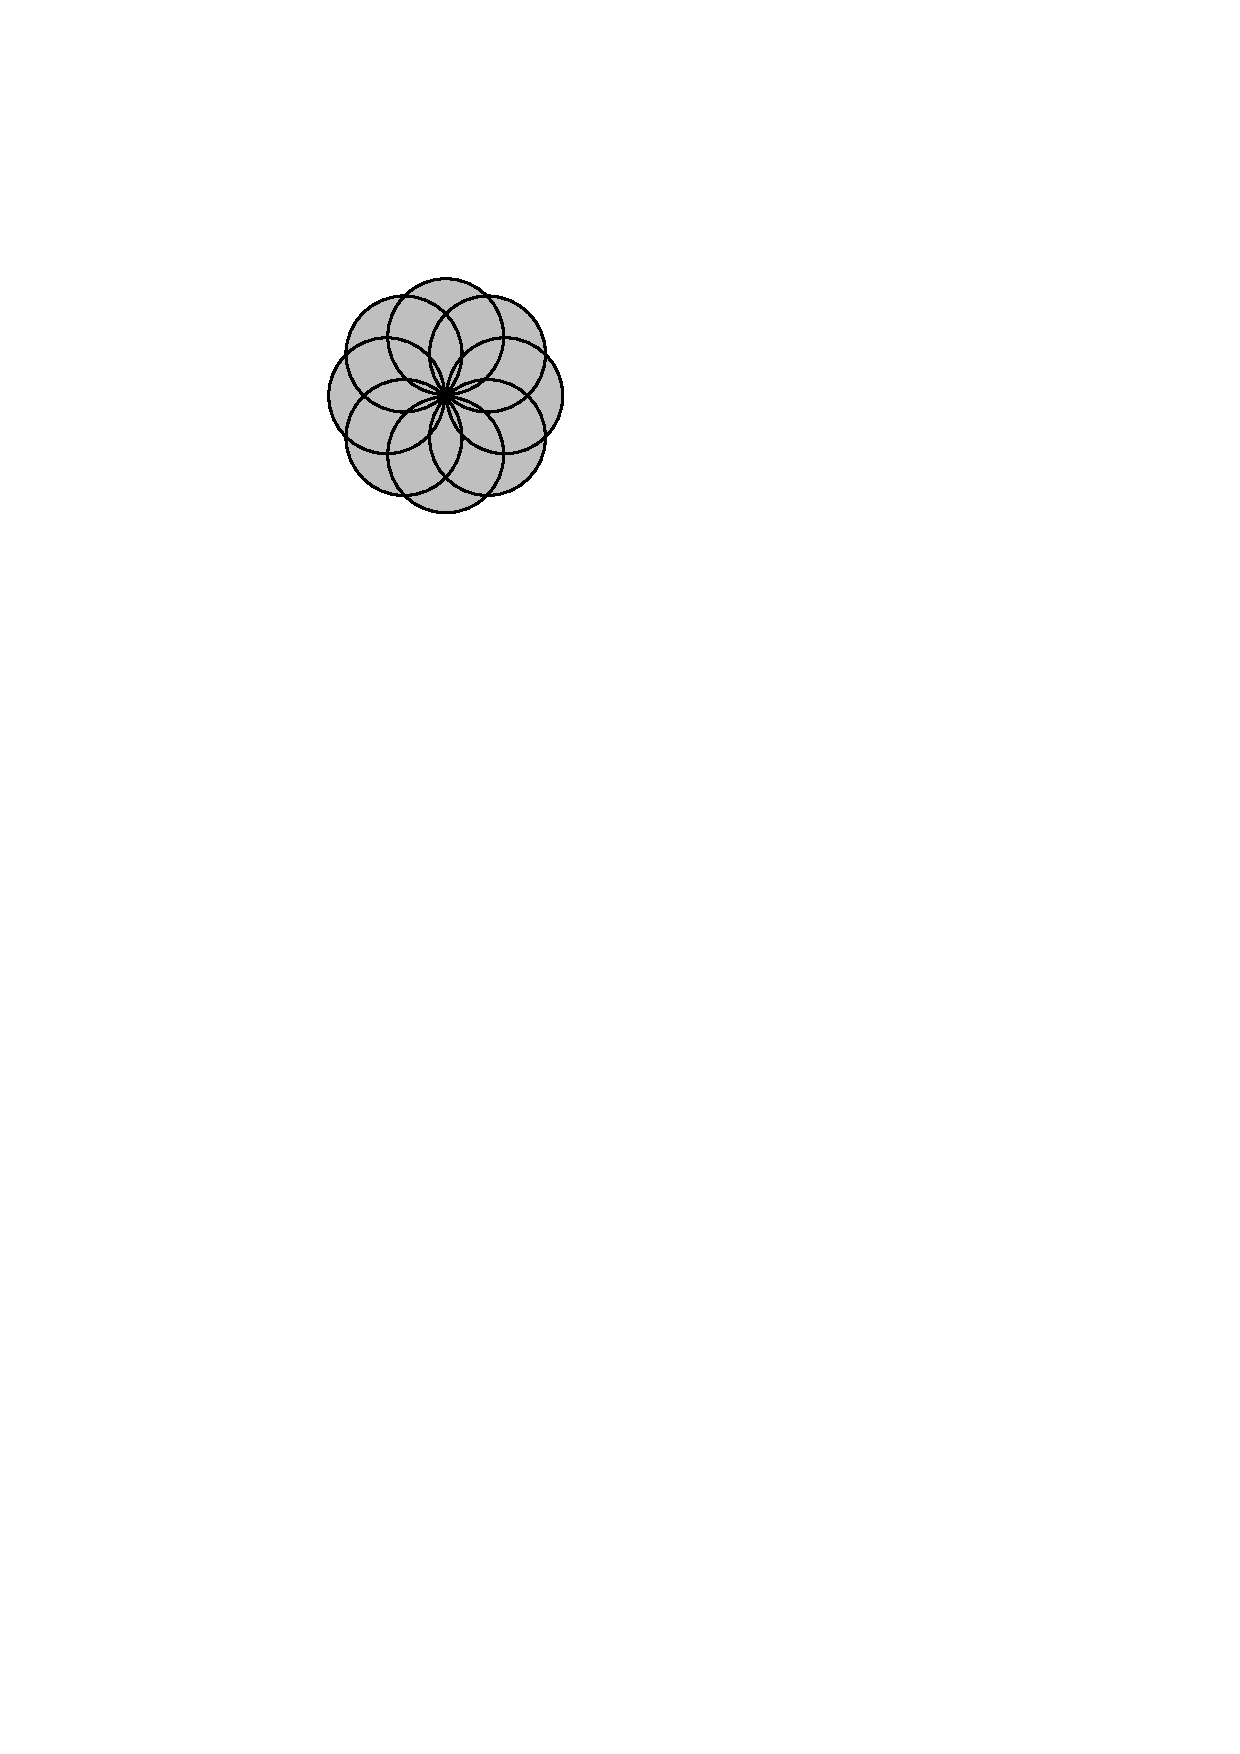
\includegraphics{Boolean_set_operations_2/fig/disks}
    \end{center}
%    Union of disks.
  \end{minipage}
\vspace{2pt}
}

\ccIncludeExampleCode{../examples/Boolean_set_operations_2/ex_set_union.C}
